\documentclass[conference]{IEEEtran}
\IEEEoverridecommandlockouts{}

\usepackage{cite}
\usepackage{amsmath,amssymb,amsfonts}
\usepackage{algorithmic}
\usepackage{graphicx}
\usepackage{textcomp}
\usepackage{xcolor}
\usepackage{hyperref}
%% ODE handling
\usepackage{diffcoeff}
\usepackage{booktabs}
%% The SI units alignment
\usepackage{siunitx}

\def\BibTeX{{\rm B\kern-.05em{\sc i\kern-.025em b}\kern-.08em
 T\kern-.1667em\lower.7ex\hbox{E}\kern-.125emX}}

\newcommand{\ui}[2]{#1_{\mathrm{#2}}}
\newcommand{\uis}[2]{#1^{\mathrm{#2}}}
\newcommand{\coo}{\ensuremath{\mathrm{CO_2}}}
\newcommand{\chho}{\ensuremath{\mathrm{CH_2O}}}

\begin{document}

\title{Carbon Neutral Greenhouse: Economic Model Predictive Control Framework for Education
    \thanks{The authors gratefully acknowledge the contribution of the Program to support young researchers under the project Adaptive and Robust Change Detection for Enhanced Reliability in Intelligent Systems. The authors gratefully acknowledge the contribution of the Scientific Grant Agency of the Slovak Republic under the grants 1/0490/23, 1/0297/22, and 1/0691/21. This research is funded by the Horizon Europe under the grant no. 101079342 (Fostering Opportunities Towards Slovak Excellence in Advanced Control for Smart Industries).}
}

\author{\IEEEauthorblockN{Marek Wadinger, Rastislav F\'aber, Erika Pavlovi\v cov\'a, Radoslav Paulen}
    \IEEEauthorblockA{\textit{Faculty of Chemical and Food Technology} \\
        \textit{Slovak University of Technology in Bratislava}\\
        Bratislava, Slovakia \\
        \texttt{marek.wadinger@stuba.sk}}
}

\maketitle

\begin{abstract}
    This paper presents a comprehensive framework aimed at enhancing education in modeling, optimal control, and nonlinear Model Predictive Control~(MPC) through a practical greenhouse climate control model. The framework includes a detailed mathematical model of lettuce growth and greenhouse, which are influenced by real-time external weather conditions obtained via an application programming interface~(API). Using this data, the MPC-based approach dynamically adjusts greenhouse conditions, optimizing plant growth and energy consumption and minimizing the social cost of CO\textsubscript{2}. The presented results demonstrate the effectiveness of this approach in balancing energy use with crop yield and reducing CO\textsubscript{2} emissions, contributing to economic efficiency and environmental sustainability.
    Besides optimizing lettuce production, the framework also provides a valuable resource for making control systems education more engaging and effective. The main aim is to provide students with a hands-on platform to understand the principles of modeling the complexity of MPC and the trade-offs between profitability and sustainability in agricultural systems. This framework uses real-world data and dynamic simulations to provide students with hands-on experience with advanced control theories, helping them to understand the control theory better, connecting it to practical implementation, and developing their problem-solving skills. The educational platform for this framework can be accessed at \url{ecompc4greenhouse.streamlit.app}.
\end{abstract}

\begin{IEEEkeywords}
    Model Predictive Control, Lettuce Growth Optimization, Greenhouse Energy Management, Precision Agriculture, Economic Yield Optimization
\end{IEEEkeywords}

\section{Introduction}

% - General introduction (why is it important that we do what we do)
In the rapidly evolving field of engineering, there is an increasing demand for graduates who possess not only theoretical knowledge but also practical skills applicable in real-world scenarios. Technical university education requires a solid foundation in theory coupled with opportunities for practical learning, often gained through participation in projects, solving real-world problems, and conducting experiments. The benefits of using interactive tools in control theory instruction have been highlighted in previous works, such as those by~\cite{Emami1991} and~\cite{Guzman2013}. Importantly, practical learning does not always rely on physical experiments with costly equipment in labs; simulations and interactive tasks can serve as effective alternatives, offering new learning opportunities.

Current farming practices are labor-intensive, seasonal, constrained by irrigation, and rely on subsidized inputs, leading to environmental issues such as eutrophication, deforestation and soil degradation. With nearly 70\% of global water resources consumed by agriculture~\cite{Debroy2024}, greenhouses offer a solution by providing controlled environments that enhance productivity beyond what open-field cultivation can achieve. However, these systems face challenges, such as fluctuating internal temperatures that can harm crops. Effective climate management, through controlled ventilation and heating, is essential for maintaining optimal conditions and improving yields~\cite{Wu2019}.

% - Concrete introduction (what is the state of the art in the domain)
Solar radiation is vital for plant growth and energy generation in greenhouses. Key metrics include Global Horizontal Irradiance~(\(GHI\)) and Photosynthetically Active Radiation~(\(PAR\)), the latter directly influencing photosynthesis. Recent research has advanced models for accurate \(PAR\) prediction~\cite{Iddio2020, MaLu2022}, while various control methods have been explored to enhance greenhouse environments and resource use efficiency. Adaptive control adjusts parameters based on real-time feedback, enabling dynamic responses to changing conditions~\cite{Tian2022}. Nonlinear feedback control addresses system complexity through advanced algorithms, improving overall system responsiveness and stability~\cite{Bood2023}. Fuzzy control effectively manages imprecise data and uncertainties, making it suitable for fluctuating environmental variables~\cite{smartcities7030055}. Robust control ensures stability despite external disturbances, contributing to reliable operation under varying conditions~\cite{Zhang2021}. Optimal control fine-tunes actions to achieve the best possible outcomes under specific constraints~\cite{Debroy2024, SVENSEN2024108578}. Despite their strengths, these approaches often require complex implementation, with frequent adjustments leading to higher energy consumption and wear on actuators.

While PID controllers are valued for their simplicity and effectiveness, IoT and machine learning are also being integrated into greenhouse control, as demonstrated by Wang et al.~\cite{Wang2024}, who combined these technologies with PID for real-time monitoring. Nonetheless, managing greenhouse systems using PID can be challenging due to the need for multiple controllers and extensive tuning. This process is time-consuming and case-dependent, often lacking guaranteed optimal results.

Consequently, MPC has emerged as a preferred approach for greenhouse climate control~\cite{Hu2022}, enabling continuous adjustment of setpoints through sample-by-sample online optimization. This approach, however, increases computational demands.

% - Educational context and relevance
Integrating advanced control techniques into education has become increasingly important. Recent studies~\cite{WangEducation2024, Zakova2024} have shown that web-based simulation platforms significantly enhance students' problem-solving skills by bridging the gap between theory and practice. Inspired by this approach, our framework aims to provide a similar educational experience within greenhouse climate control, focusing on modeling, optimal control, and Nonlinear Economic Model Predictive Control~(NEMPC).

% - Presentation of our contribution
This study presents a web interface for optimizing greenhouse climate control, to achieve enhanced crop yields, energy efficiency and reduction in \coo\ emissions. Utilizing principles of thermodynamics, fluid dynamics, and mass transfer, along with real weather and carbon intensity forecasts we developed a simulation environment employed by NEMPC to adjust ventilation, heating, humidification, and \coo\ enrichment in real-time. Beyond technical contributions, the framework serves as an educational tool, allowing students to engage with real-world data and explore the economic and sustainability trade-offs in agricultural systems. Thus, this versatile platform enhances control education by combining theoretical concepts with practical skills in automatic control.

\section{Greenhouse Climate Model}\label{sec:greenhouse}
In this section we provide a mathematical model of the greenhouse environment, focusing on wind, temperature, humidity, and \coo\ concentration dynamics that implements the GES software~\cite{rmward61_2019} based on the Gembloux Dynamic Greenhouse Climate Model~\cite{GDGCM} and work by Vanthoor~\cite{Vanthoor2011}.

\begin{figure}
    \centering
    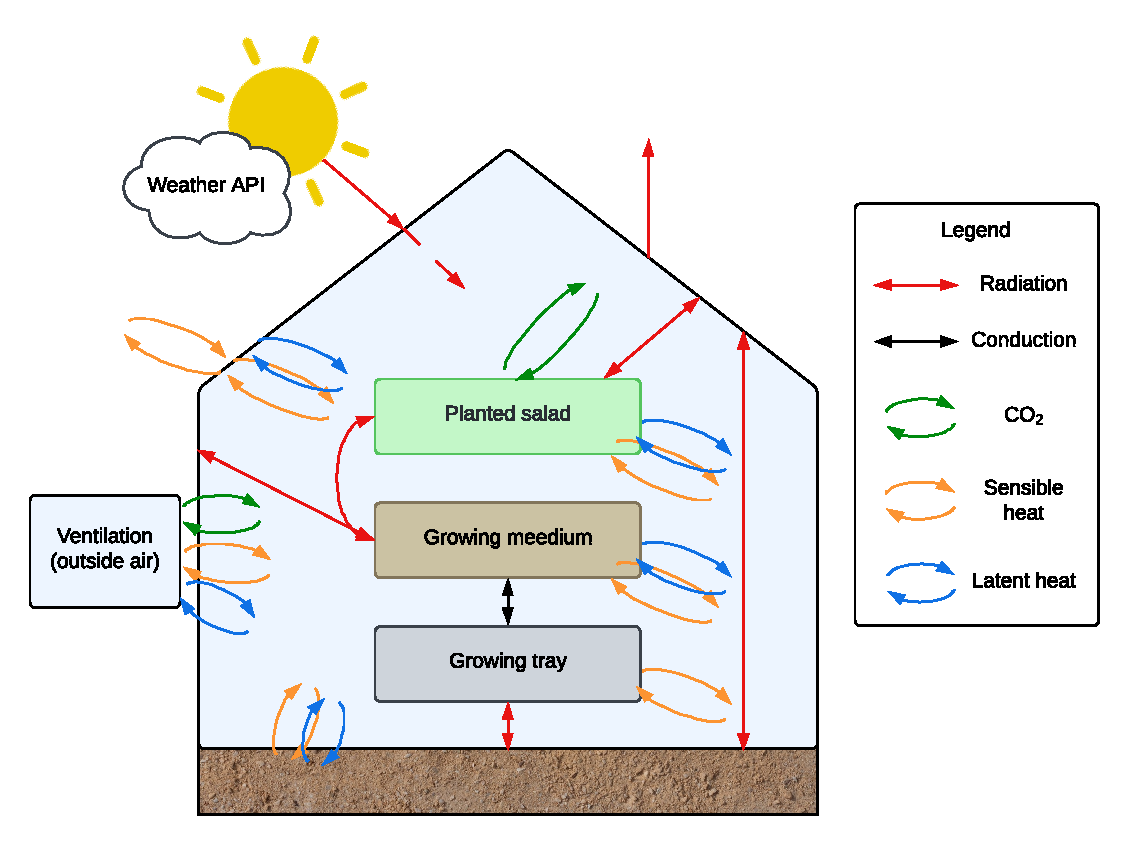
\includegraphics[width=.5\textwidth]{images/diagram.pdf}
    \caption{A simplified diagram of the heat, mass and \coo\ exchanges modelled within the framework. Image adapted from~\cite{rmward61_2019}.}\label{fig:diagram}
\end{figure}

\subsection{Temperature Dynamics}\label{subsec:temperature}

The temperature dynamics inside the greenhouse are modeled by considering the energy exchange due to convection, radiation, and conduction --- Fig.~\ref{fig:diagram}. The temperatures of different components (e.g., cover, internal air, vegetation, tray, etc.) are described using the following equations.

The convective heat transfer between two surfaces is given by:
\begin{equation}
    \text{Nu} = \max \left( \text{Nu}_G, \text{Nu}_R \right),
\end{equation}
where \(\text{Nu}_G\) and \(\text{Nu}_R\) are the Nusselt numbers for free and forced convection, respectively:
\begin{align}
    \text{Nu}_G & = 0.5  {\left( \frac{\text{Gr}}{10^5} \right)}^{0.25} + 0.13  {\left(\frac{\text{Gr}}{10^5}\right)}^{0.33}, \\
    \text{Nu}_R & = 0.6  {\left(\frac{\text{Re}}{20000}\right)}^{0.5} + 0.032  {\left(\frac{\text{Re}}{20000}\right)}^{0.8},
\end{align}
where Re represents the Reynolds number, and Gr represents the Grashof number.

The heat flux due to convection is then calculated as:
\begin{equation}
    Q_{\text{conv}} = A_{\text{c}}\, \text{Nu}\, \lambda_{\text{air}} \frac{T_1 - T_2}{d_{\text{c}}},
\end{equation}

where \(A_c\) and \(d_c\) represent the and the characteristic length of a compartment, respectively, and \(\lambda_{air}\) is the approximate thermal conductivity for air at room temperature.

The radiative heat transfer between two surfaces is described by:
\begin{equation}
    Q_{\text{rad}} = \frac{\varepsilon_1  \varepsilon_2}{1 - \rho_1  \rho_2  F_{12}  F_{21}}  \sigma  A_1  F_{12}  \left( T_1^4 - T_2^4 \right),
\end{equation}
where \(\sigma \) is the Stefan-Boltzmann constant, \(F_{12}\) is the view factor from surface 1 to surface 2, \(T_1\) and \(T_2\) representing the temperatures of the surfaces, and \(\varepsilon \) and \(\rho \) are the emissivity and reflectivity of the surfaces, respectively.

The conductive heat transfer through a medium is given by:
\begin{equation}
    Q_{\text{cond}} = \frac{A \lambda_{\text{c}}}{d_\text{l}} (T_1 - T_2),
\end{equation}
where \(\lambda_{\text{c}} \) is the thermal conductivity of a compartment, and \(d_{\text{l}}\) is the thickness of the conducting layer.

\subsection{Humidity Dynamics}\label{subsec:humidity}

The humidity within the greenhouse is modeled by considering the mass transfer of water vapor. The specific humidity is calculated as:
\begin{equation}
    \text{SH} = \exp\left(11.56 - \frac{4030}{T + 235}\right).
\end{equation}
The moisture content in the air is given by:
\begin{equation}
    C_w = \text{SH} \times \rho_{\text{air}},
\end{equation}
where \(\rho_{\text{air}}\) is the density of air.

The mass transfer of water vapor due to convection is:
\begin{equation}
    Q_{v} = \frac{A  H_{\text{fg}}}{\rho  c}  \frac{\text{Sh}}{\text{Le}}  \frac{\lambda}{d}  \left( C - C_{\text{sat,}T} \right),
\end{equation}
where \(H_{\text{fg}}\) is the latent heat of vaporization, \(\text{Sh}\) is the Sherwood number, and \(\text{Le}\) is the Lewis number, \(\lambda \) is the thermal conductivity, \(d\) is the characteristic length, \(A\) is the heat exchange surface area, \(\rho \) is the density of the vapor, \(c\) is the specific heat capacity, \(C\) is the actual vapor concentration --- referring  to the amount of water vapor present in the air in a given volume --- and \(C_{\text{sat,}T}\) is the saturated vapor concentration at temperature \(T\).

\subsection{Carbon Dioxide Concentration Dynamics}

The \coo\ concentration within the greenhouse is affected by photosynthesis and external conditions. The external \coo\ concentration is computed as:
\begin{equation}
    C_{\text{ext}} = \frac{4 \times 10^{-4}  M_c  P_{\text{atm}}}{R  T_{\text{ext}}},
\end{equation}
where \(M_c\) is the molar mass of \coo, \(P_{\text{atm}}\) is the atmospheric pressure, \(R\) is the gas constant, and \(T_{\text{ext}}\) is the external air temperature in Kelvin.

The internal \coo\ concentration in parts per million (ppm) is given by:
\begin{equation}
    C_{\text{int, ppm}} = \frac{C_c  R  T_i}{M_c  P_{\text{atm}}} \times 10^6,
\end{equation}
where \(C_c\) is the \coo\ density, and \(T_{\text{in}}\) is the internal air temperature in Kelvin.

The greenhouse climate model integrates the physical models of temperature, humidity, and \coo\ concentration into a dynamic system represented by a state vector \(\mathbf{z}\) = [\(T_c, T_i, T_v, T_m, T_p, T_f, T_s, C_w, C_c, x_{\text{sdw}}, x_{\text{nsdw}}\)] with dimension (11, 1), and input vector \(\mathbf{u}\) = [\(Q_{\text{heater}}, R_{\text{fan}}, V_{\text{humid}}, G_{\coo} \)] with dimension (4, 1) for the heating power, ventilation, humidification, and \coo\ enrichment. The \(T_c\) represents the cover temperature, \(T_i\) the internal air temperature, \(T_v\) the planted salad temperature, \(T_m\) the growing medium temperature, \(T_p\) the tray temperature, \(T_f\) the floor temperature, and \(T_s\) the temperature of the soil layer. Additionally, \(C_w\) denotes the density of water vapor, \(C_c\) the \coo\ density, \(x_{\text{sdw}}\) the structural dry weight of the plant, and \(x_{\text{nsdw}}\) the non-structural dry weight of the plant.
% RP: Cloveka by zaujimalo ako sa dostane k rovniciam dynamiky. Nie je tu uvedene nic k rychlosti rastu salatu.

\subsection{Actuation Control Systems}
In our implementation, actuators operate by converting an input control signal from the system into the appropriate mechanical energy required to regulate environmental variables~\cite{Butterfield2018}. These actuators serve to maintain optimal conditions for crop growth by regulating temperature, humidity, ventilation, and \coo\ concentration. Each actuator's functionality is modeled to simulate its contribution to the overall energy balance, operating costs, and \coo\ emissions of the greenhouse. Below, we describe the main equations used to model these actuators, summarized in Table~\ref{tab:actuators}.

\begin{table}
    \centering
    \caption{Summary of Actuator Model Parameters}\label{tab:actuators}
    \begin{tabular}{lcc}
        \toprule
        Actuator        & Label                   & Unit                   \\
        \midrule
        Heater          & \( Q_{\text{heater}} \) & W                      \\
        Fan             & \( R_{\text{fan}} \)    & m\textsuperscript{3}/s \\
        Humidifier      & \( V_{\text{humid}} \)  & l/h                    \\
        \coo\ Generator & \( G_{\coo} \)          & kg/h                   \\
        \bottomrule
    \end{tabular}
\end{table}


We model the actuators by adjusting the control signal, \( u(t) \), which ranges from 0 to 100\%, where 0\% represents no activation, and 100\% corresponds to the maximum actuation level. The actuation level, \( a(u) \), is then calculated as:
\begin{equation}
    a(u) = \frac{u}{100}  a_{\text{max}},
\end{equation}
where \( a_{\text{max}} \) represents the scale of the specific actuator, such as the maximum heating power or airflow.

The \textbf{power consumption} of each actuator, \( P(u) \), is determined by:
\begin{equation}
    P(u) = \frac{p_{\text{unit}}}{\eta}  a(u),
\end{equation}
where \( p_{\text{unit}} \) is the power per unit of actuation, and \( \eta \) represents the efficiency of the actuator.

The \textbf{total energy cost}, \( C_{\text{energy}}(u) \), in EUR is calculated as:
\begin{equation}
    C_{\text{energy}}(u) = \frac{E_{\text{cost}}  \Delta t}{1,000 \, 3,600}  P(u),
\end{equation}
where \( E_{\text{cost}} \) is the cost of energy in EUR per kWh, and \( \Delta t \) is the time step in seconds.

The \textbf{\coo\ emissions}, \( E_{\coo}(u) \), generated by each actuator are given by:
\begin{equation}
    E_{\coo}(u) = \frac{I_{\coo}  \Delta t}{1,000  \, 3,600}  P(u),
\end{equation}
where \( I_{\coo} \) is the carbon intensity in g\coo\ eq/kWh~\cite{ElectricityMaps2022}. The associated cost of these emissions is:
\begin{equation}
    C_{\coo}(u) = C_{\coo\text{cost}}  E_{\coo}(u),
\end{equation}
where \( C_{\coo\text{cost}} \) is the social cost of \coo\ in EUR/g\coo\ eq.\\

The \textbf{heater actuator}'s heating power, \( Q_{\text{heater}} \), is determined based on the desired setpoint temperature, \( T_{\text{sp}} \), and air volume of the greenhouse, \( \Omega \):
\begin{equation}
    Q_{\text{heater}} = \rho_{\text{air}}  c_{\text{air}}  \Omega  (T_{\text{sp}} - T_{\text{ambient}})  \frac{Q_{\text{air}}}{3600},
\end{equation}
where \( \rho_{\text{air}} \) is the density of air, \( c_{\text{air}} \) is the specific heat capacity of air, and \( Q_{\text{air}} \) represents the fresh air exchange rate per hour.

The \textbf{fan actuator} controls the air exchange rate. The ventilation rate, \( R_{\text{fan}} \), is based on the air changes per hour (\( \text{ACPH} \)) --- the number of times that the total air volume in a room or space is completely removed and replaced in an hour --- and greenhouse volume \( \Omega \):
\begin{equation}
    R_{\text{fan}} = \Omega \frac{\text{\( \text{ACPH} \)}}{3600}.
\end{equation}

The \textbf{humidifier actuator} controls the humidity level within the greenhouse. The humidification rate, \( V_{\text{humid}} \), is calculated as:
\begin{equation}
    V_{\text{humid}} = \Omega \frac{\phi_{a, 80 - 40}}{\rho_{\text{water}}},
\end{equation}

where \( \phi_{a, 80 - 40} \) the maximum change in absolute humidity per hour which corresponds to difference between the absolute humidity at 80\% and 40\% relative humidity at a temperature of 20\( ^\circ \)C, and \( \rho_{\text{water}} \) is the density of water.

The \textbf{\coo\ actuator} increases the \coo\ concentration within the greenhouse. The \( G_{\coo} \) is based on the desired change of the \coo\ density per hour, \( \dot{c}_{co2} \) and air volume:
\begin{equation}
    G_{\coo} = \dot{c}_{co2}  V,
\end{equation}
where \( G_{\coo} \) is the \coo\ generation in kg/h.


\section{Lettuce Growth Model}\label{sec:lettuce_growth}
The growth of lettuce is be modeled using a dynamic system of equations that captures the behavior of both structural (SDW) and non-structural dry weight (NSDW) of the plant~\cite{VANHENTEN199455}. The dynamics of conversion of  model is influenced by environmental factors such as temperature, light (PAR), and \coo\ concentration. The model equations are parameterized using well-established constants from the literature and adapted for dynamic simulation. For the complete list of parameters and their values with references, see source code repository~\cite{Wadinger2024}.

\subsection{Dynamic Growth Equations} The dynamic equations for structural and non-structural dry weight are given by the following differential equations. The rate of change of structural dry weight is governed by the specific growth rate \( \ui{r}{gr} \) and is modeled as:

The state equations governing the system are defined as:

\[
    \diff{\ui{x}{sdw}}{t} = \ui{r}{gr} \ui{x}{sdw}
\]
\[
    \begin{aligned}
        \diff{\ui{x}{nsdw}}{t} & = c_{\chho/\coo} \ui{f}{phot} - \ui{r}{gr} \ui{x}{sdw} - \ui{f}{resp}                   \\
                               & \quad - \left( \frac{1 - Y_{\chho/\coo}}{Y_{\chho/\coo}} \right) \ui{r}{gr} \ui{x}{sdw}
    \end{aligned}
\]

where \( c_{\chho/\coo} \) is the conversion factor representing the efficiency with which plants convert absorbed carbon dioxide into biomass, \( Y_{\chho/\coo} \) is the yield, \( \ui{f}{phot} \) is the gross photosynthesis, and \( \ui{f}{resp} \) is the maintenance respiration.

The physiological processes that are included in lettuce growth model are described in detail in~\cite{VANHENTEN199455}. These processes include growth, respiration, photosynthesis, and canopy conductance.

\subsection{Specific Growth Rate} The specific growth rate \( \ui{r}{gr} \) describes the rate at which the structural biomass (SDW) accumulates in response to the non-structural dry weight (NSDW) available in the plant. This process is temperature-dependent, with the growth rate scaling based on a plants temperature sensitivity, which adjusts the growth response as the canopy temperature changes. The non-structural dry weight provides a reservoir of energy for structural growth, and the efficiency of this conversion is central to the plant's overall biomass accumulation.

\subsection{Maintenance Respiration} The maintenance respiration rate \( \ui{f}{resp} \) accounts for the energy expenditure required to sustain the plant's basic metabolic functions. This respiration process is divided between the shoot and root components, where each part has its own maintenance respiration rate, scaled to the dry mass of the plant. Respiration demands increase as temperatures rise, reflecting the greater energy requirements at higher temperatures. Respiration is a key factor in determining how much energy is left for growth, as it consumes a portion of the energy generated from photosynthesis.

\subsection{Gross Photosynthesis} The photosynthesis model determines the gross canopy photosynthesis rate \( \ui{f}{phot} \), which represents the total \coo\ assimilation by the plant. This is primarily driven by the maximum \coo\ assimilation rate, which depends on the incident photosynthetically active radiation (PAR), \coo\ concentration, and the canopy's light-use efficiency. The leaf area index and extinction coefficient further influence how efficiently light is absorbed across the canopy. Canopy conductance plays a critical role in this process by regulating the rate at which \coo\ diffuses into the leaf. The combined effect of boundary layer conductance, stomatal conductance, and carboxylation conductance ensures that \coo\ reaches the sites of photosynthesis efficiently. Carboxylation conductance itself is temperature-dependent, following a quadratic relationship with temperature, reflecting how enzymatic activity is influenced by environmental conditions.


% \subsection{Specific Growth Rate}

% The specific growth rate \( \ui{r}{gr} \) is defined as:

% \[
%     \ui{r}{gr} = \ui{c}{gr, max} \frac{\ui{x}{nsdw}}{\ui{c}{\gamma} \ui{x}{sdw} + \ui{x}{nsdw}} \ui{c}{qr, Q10}^{\left(\frac{\ui{u}{T} - 20}{10}\right)}
% \]

% where \( \ui{u}{T} \) is the canopy temperature, \( \ui{c}{gr, max} \) is the saturated growth rate at 20°C, \( \ui{c}{\gamma} \) is the growth rate coefficient, and \( \ui{c}{qr, Q10} \) is the growth sensitivy to change in temperature by 10\( ^\circ \)C.

% \subsection{Respiration Model}

% The maintenance respiration rate \( \ui{f}{resp} \) is defined as:

% \[
%     \ui{f}{resp} = \left( \ui{c}{resp, s} (1 - \ui{c}{\tau}) \ui{x}{sdw} + \ui{c}{resp, r} \ui{c}{\tau} \ui{x}{sdw} \right) \ui{c}{resp, Q10}^{\left( \frac{\ui{u}{T} - 25}{10} \right)}
% \]

% where the \( \ui{c}{resp, s} \) and \( \ui{c}{resp, r} \) are the shoot and root maintenance respiration rate at 25°C, \( \ui{c}{\tau} \) is the root dry mass ratio, and \( \ui{c}{qr, Q10} \) is the respiration sensitivy to change in temperature by 10\( ^\circ \)C.

% \subsection{Photosynthesis Model}

% The photosynthesis model is divided into two parts: the maximum \coo\ assimilation rate and the gross canopy photosynthesis. The maximum \coo\ assimilation rate \( \ui{f}{phot, max} \) is given by:

% \[
%     \ui{f}{phot, max} = \frac{\epsilon \ui{u}{PAR} \ui{g}{\coo} \ui{c}{\omega} (\ui{u}{\coo} - \Gamma)}{\epsilon \ui{u}{PAR} + \ui{g}{\coo} \ui{c}{\omega} (\ui{u}{\coo} - \Gamma)}
% \]

% where the \( \ui{u}{PAR} \) is the incident photosynthetically active radiation, \( \ui{u}{\coo} \) is the \coo\ concentration, \( \epsilon \) is the light-use efficiency, \( \ui{g}{\coo} \) is the canopy conductance to \coo\ diffusion, \( \ui{c}{\omega} \) is the density of \coo\ in air, and \( \Gamma \) is the \coo\ compensation point.

% The gross canopy photosynthesis \( \ui{f}{phot} \) is expressed as:

% \[
%     \ui{f}{phot} = \left( 1 - \exp\left( -\ui{c}{K} \ui{c}{LAR} (1 - \ui{c}{\tau}) \ui{x}{sdw} \right) \right) \ui{f}{phot, max}
% \]

% where \( \ui{c}{K} \) is the extinction coefficient, and \( \ui{c}{LAR} \) is the structural leaf area ratio.

% \subsection{Canopy Conductance}

% The canopy conductance to \coo\ diffusion \( \ui{g}{\coo} \) is given by:

% \[
%     \ui{g}{\coo} = \frac{1}{\left( \frac{1}{\ui{g}{BND}} + \frac{1}{\ui{g}{STM}} + \frac{1}{\ui{g}{CAR}} \right)}
% \]

% where \( \ui{g}{BND} \) is the boundary layer conductance, \( \ui{g}{STM} \) is the stomatal resistance, and \( \ui{g}{CAR} \) is the carboxylation conductance,

% \subsection{Carboxylation Conductance}

% The carboxylation conductance \( \ui{g}{CAR} \) is modeled as a quadratic function of temperature:

% \[
%     \ui{g}{CAR} = \ui{c}{CAR1} \ui{u}{T}^2 + \ui{c}{CAR2} \ui{u}{T} + \ui{c}{CAR3}
% \]

% where:
% - \( \ui{c}{CAR1} \), \( \ui{c}{CAR2} \), and \( \ui{c}{CAR3} \) are carboxylation parameters dependent on temperature.


\section{Nonlinear economic model predictive control}\label{sec:mpc}

A nonlinear economic model predictive control~(NEMPC) is adopted to maximize the profit from growing lettuce in a greenhouse. The objective of the proposed MPC for greenhouse control is to optimize the economic performance of the greenhouse system by controlling its actuators, such as heating, ventilation, and \coo\ injection. This is achieved by maximizing lettuce yield while minimizing operating costs over a finite prediction horizon. The NEMPC framework incorporates the dynamics of the greenhouse and time-varying external conditions such as weather.

\subsection{System Dynamics}\label{subsec:mpc_dynamics}

The greenhouse system is modeled by a set of nonlinear state equations (see Section~\ref{sec:greenhouse}) that describe the evolution of the greenhouse states, such as temperature, humidity, and biomass. The discrete-time nonlinear system is given by:
\begin{equation}
    x(t+1) = f\left( x(t), u(t), p(t) \right),
\end{equation}
where \(x(t) \in \mathbb{R}^{n_x}\) represents the state vector at time step \(t\), \(u(t) \in \mathbb{R}^{n_u}\) represents the control input vector (actuators), and \(p(t)\) are time-varying parameters that include external climate conditions such as temperature, radiation, and humidity.

\subsection{Economic Objective Function}\label{subsec:mpc_objective}

The goal of the economic MPC is to maximize the revenue from lettuce production while minimizing the costs associated with actuator use. The objective function is composed of two terms: the profit from biomass accumulation and the costs of actuators.

The revenue from lettuce production is proportional to the change in biomass between the initial state and the current state, expressed as:
\begin{equation}
    R(t) = P_L  \frac{(\ui{x}{sdw}(t) + x_{\mathrm{nsdw}}(t)) - (x_{0, \mathrm{sdw}} + x_{0, \mathrm{nsdw} })}{\rho_{dw}}  A_c,
\end{equation}
where \(P_L\) is the price of lettuce per gram, \(A_c\) is the cultivated area, \(\ui{x}{sdw}\) and \(x_{\mathrm{nsdw}}\) are the biomass-related states, and \(rho_{dw}\) stands for dry-to-wet ratio.

In addition, the cost of operating the actuators at each time step is given by:
\begin{equation}
    C_u(t) = \sum_{i} \left( C_{\text{energy}}(u_i(t)) + C_{\coo}(u_i(t)) \right),
\end{equation}
where \(C_{\text{energy}}(u_i(t))\) is the cost associated with the actuator signal \(u_i(t)\) and \(C_{\coo}(u_i(t))\) represents the cost related to \coo\ emissions from the actuator.

Thus, the total cost at each time step is:
\begin{equation}
    l_t = -R(t) + C_u(t).
\end{equation}

\subsection{Optimization Problem Formulation}

The objective of the nonlinear economic MPC is to minimize the sum of the stage costs \(l_t\) over a finite prediction horizon \(N\), subject to system dynamics and constraints. The optimization problem is formulated as follows:
\begin{equation}
    \min_{{\{u(t)\}}_{t=0}^{N-1}} \sum_{t=0}^{N-1} l_t(x(t), u(t)),
\end{equation}
subject to:
\begin{align}
    x(t+1)   & = f(x(t), u(t), p(t)),                                    \\
    u_{\min} & \leq u(t) \leq u_{\max}, \quad \forall t = 0, \dots, N-1, \\
    x_{\min} & \leq x(t) \leq x_{\max}, \quad \forall t = 0, \dots, N,   \\
    x(0)     & = x_{\text{initial}}.
\end{align}
Here, \(x_{\min}\) and \(x_{\max}\) represent the bounds on the state variables, and \(u_{\min}\) and \(u_{\max}\) define the bounds on the control inputs, i.e., actuator signals.

\subsection{Time-Varying Parameters}

The external climate conditions are modeled as time-varying parameters~(TVP), which influence the system dynamics. These parameters include variables such as outdoor temperature, solar radiation, and humidity, and are provided by real-time weather data. The parameters are incorporated into the state equations, influencing the evolution of the greenhouse states.

\section{Educational Web Interface}
Figure~\ref{fig:web} demonstrates the interactive web-based educational tool. Via four layers of customization of the greenhouse, users may learn the main benefits of optimal control and challenges related to non-linearity. The first layer is the greenhouse structure, where the user can select the shape of the greenhouse, affecting the energy exchange with the environment and suggested scaling of the actuation units.

The second layer is the orientation and location of the greenhouse, which affects the solar radiation and the weather conditions. Here, we establish a connection to weather and carbon intensity forecast APIs to provide real-time data along with forecasts and history replays.

The third layer is the actuation units, where the user can overwrite the suggested scaling and select the actuators for the heating, ventilation, humidification, and \coo\ enrichment. Meanwhile, the fourth layer is the control strategy, where the user can influence the control parameters, including the objective function and constraints of the economic MPC controller.

While the user is customizing the greenhouse, the web interface provides real-time feedback. The user can also simulate the greenhouse operation over a selected period of time and analyze the results in terms of energy consumption, crop yield, and economic output.

\begin{figure}\label{fig:web}
    \centering
    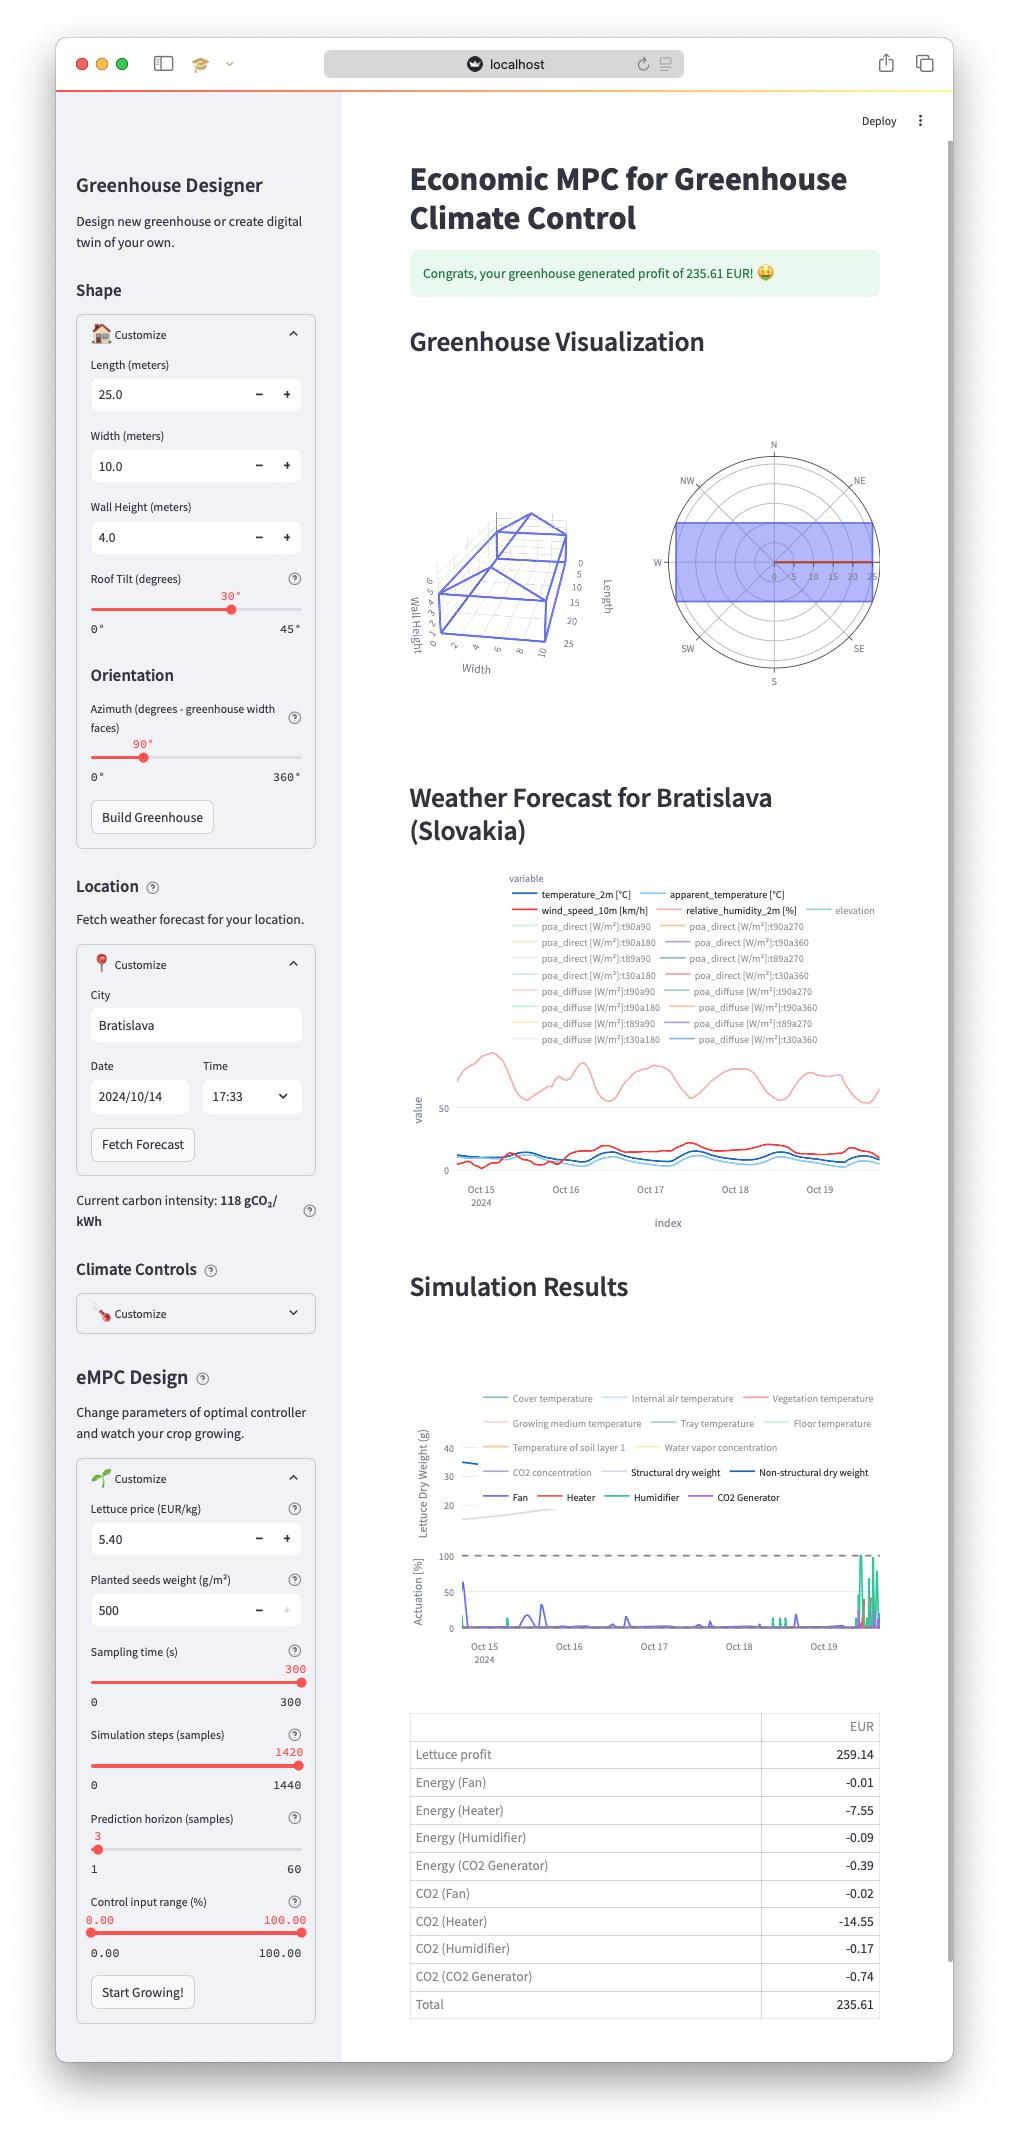
\includegraphics[width=.5\textwidth]{figures/webpage.png}
    % RP: Prilis vela bieleho miesta na okrajoch.
    \caption{Interactive web-based educational tool designed to teach students the principles of NEMPC applied to greenhouse climate management. The sidebar shows customization layers. The main window displays the greenhouse structure, orientation, weather forecast, simulation results, and cost-profit analysis.}
\end{figure}

\section{Results}
% Comparison of controlled greenhouse vs greenhouse without actuation
In the first set of simulations, we analyzed the nonlinear behavior of the greenhouse under varying climate conditions and steps in actuation. We observed how different actuations influence the growth of the structural and non-structural dry weight of the plant. The simulations were run under a mild climate of Bratislava (Slovakia), from 11\textsuperscript{th} October for a 24-hour window. Figure~\ref{fig:steps} shows that under given climate conditions,
the influence of ventilation and humidification is insignificant on growth as compared to the situation where no change in actuation was applied.
Nevertheless, it has a positive effect on convection and the overall transfer of energy. Meanwhile, intense heating positively influences the conversion of non-structural dry weight into structural dry weight but does not influence the overall non-structural dry weight buildup.~\coo\ enrichment has a significant impact on non-structural plant growth.

\begin{figure*}
    \centering
    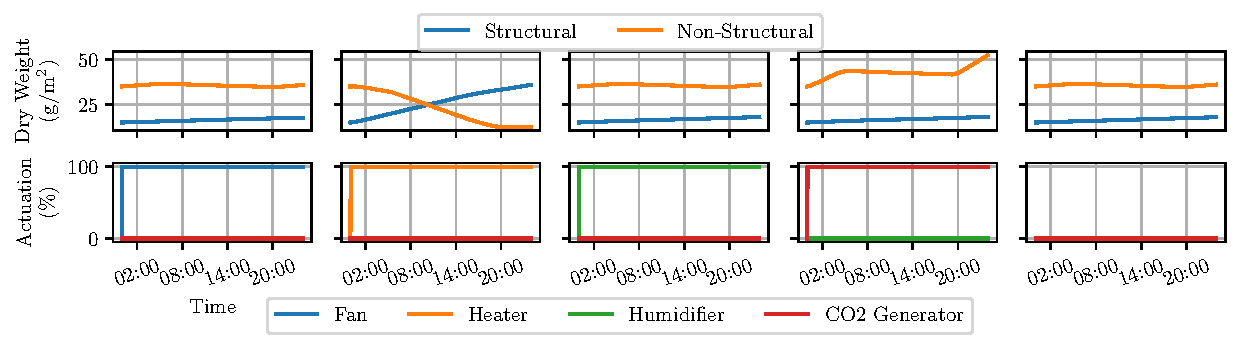
\includegraphics[width=\textwidth]{figures/step_response-outputs-2024-10-11_2024-10-26-120s.pdf}
    \caption{Responses of structural and non-structural dry weight on step changes from off to maximum in following actuations from the left to the right: ventilation, heating, humidification, and \coo\ enrichment, no step made.}\label{fig:steps}
\end{figure*}


The second set of simulations compares the performance of the proposed NEMPC algorithm with a no-control scenario. The NEMPC algorithm was configured with a prediction horizon of 10 minutes and a control horizon of 10 minutes. The simulations were run for a total of 10,801 steps, with a sampling time of 120 seconds. Results demonstrate that the proposed economic MPC algorithm increased crop yield by 9\% and increased profit by more than 4\% in just 15 days of growth.
Moreover, the cost function of the NEMPC algorithm included the social cost of the carbon intensity of the energy sources used. This addition led to a 98\% reduction in \coo\ consumption, although it caused a fourfold decrease in plant growth when compared to a scenario where the social cost of \coo\ was not minimized. This highlights a significant trade-off between economic output and the carbon intensity of the energy sources. While farmers may prioritize economic gains, the environmental impact of production deserves careful consideration.

\begin{figure}\label{fig:control}
    \centering
    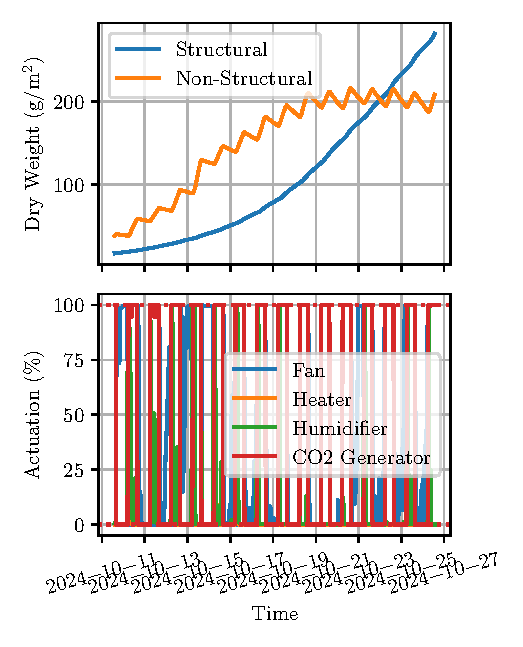
\includegraphics[width=.5\textwidth]{figures/greenhouse_control-mpc_co2-N_30-steps_10801.pdf}
    % RP: Tieto grafy by kludne zniesli znizenie vysky o polovicu na usetrenie miesta. Nie je na vrchu a na spodku prilis vela bieleho miesta?
    \caption{A simplified diagram of the heat, mass and \coo\ exchanges modeled within the framework. Image adapted from~\cite{rmward61_2019}.}
\end{figure}

\begin{table}
    \centering
    \caption{Performance comparison: NEMPC {vs. } no control.}\label{tab:comparison}
    \begin{tabular}{lS[table-format=4.2]S[table-format=4.2]S[table-format=4.2]}
        \toprule
        Parameter           & {No control} & {NEMPC (\coo\ )} & {NEMPC (\$)} \\
        \midrule
        Lettuce profit      & 858.32       & 940.19           & 4120.63      \\
        Energy (Fan)        & 0.00         & -0.03            & -0.16        \\
        Energy (Heater)     & 0.00         & -0.45            & -21.68       \\
        Energy (Humidifier) & 0.00         & -0.05            & -0.00        \\
        Energy (\coo\ Gen.) & 0.00         & -9.95            & -697.59      \\
        \coo\ (Fan)         & 0.00         & -0.08            & -0.51        \\
        \coo\ (Heater)      & 0.00         & -1.48            & -70.84       \\
        \coo\ (Humidifier)  & 0.00         & -0.17            & -0.01        \\
        \coo\ (\coo\ Gen.)  & 0.00         & -32.52           & -2279.72     \\
        \midrule
        Total               & 858.32       & 895.45           & 1050.12      \\
        \bottomrule
    \end{tabular}
\end{table}

% Educational trials
To assess the educational impact of our proposed paper, we conducted a survey among students who interacted with the web-based application. The survey measured the participants' prior knowledge and their learning outcomes in four key areas: mathematical modeling, optimal process control, economic process control, and MPC.\@

The results based on five responses show a varied range of initial expertise levels in both modeling and process control, with participants rating their skills from novice (1) to advanced (5). Despite this variation, the application demonstrated a significant educational benefit across all experience levels.

\paragraph{Low-Skilled Users}
Participants with minimal prior knowledge reported moderate improvements in understanding mathematical modeling, optimal control, and economic control, with a strong positive impact noted for MPC.\@ These results suggest that the framework is accessible to beginners and helps building foundational knowledge.

\paragraph{High-Skilled Users}
More experienced participants rated the application as highly beneficial in all four categories. They noted substantial improvements in their understanding of complex control techniques, particularly in mathematical modeling and MPC, validating the educational potential of the framework for users with advanced backgrounds.

\paragraph{General Feedback}
The participants' qualitative feedback further highlights the application's potential. Participants emphasized that with additional information, the tool could be used by a broader audience, including industrial farmers, to design and optimize greenhouse placement in practical settings. This points to the dual benefit of the application: it not only enhances student learning but could also have real-world applicability in sustainable greenhouse design.

These findings suggest that the proposed framework effectively supports educational objectives, promoting understanding across a spectrum of learners. It also has the potential to be adapted for broader use beyond educational contexts, providing valuable insights into the design of sustainable greenhouse systems.

\section{Conclusion}
This study introduces a framework that combines the Nonlinear Economic Model Predictive Control (NEMPC) with a detailed mathematical model to control the greenhouse climates, aiming to optimize lettuce growth. The provided framework utilizes real-time weather forecasts and carbon intensity data, to adjust the environmental conditions, i.e., temperature, humidity, and \coo\ levels, improving crop yields, energy efficiency, and reducing \coo\ emissions.

The main contribution of this paper is educational tool helping students to better understand nor only the control theory but also to connect it with practical, real-world challenges. Through a user-friendly web-based platform, students can engage with advanced control theories while exploring the complexities of balancing economic goals and sustainability in greenhouse management.

Student feedback has proven that the framework helps both beginning and advanced automatic control students deepen their understanding of modeling, process control, and MPC techniques. Future work could focus on including other automatic control approaches and exploring more interactive features to enrich the learning experience further.

\bibliographystyle{IEEEtran}
\bibliography{main}

\end{document}
